\section{Paragraf autorstwa Agaty Marczyk}
\begin{flushleft}
    Jednym z pierwszych modeli \textbf{Sztucznych neuronów} był model \textit{McCullocha-Pittsa}
    powstały w \textbf{1943 roku.} \underline{Model matematyczny wzór(\ref{eq1})}
    \textbf{Dodatkowa} linijka \underline{tekstu} do celów \textsc{formatowania}
    \begin{equation} \label{eq1}
        {\displaystyle s=w_{0}+\sum _{i=1}^{n}x_{i}w_{i}}
    \end{equation}
    \setlength{\parindent}{20pt}

    \section*{Sztuczne sieci neuronowe zdjęcie(\ref{fig:Neuron})}
    \textbf{tabela\ref{tab:tab1}} 

     \begin{figure}[ht]
        \centering
        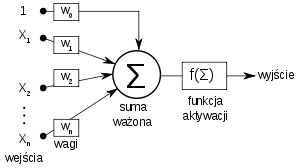
\includegraphics{pictures/300px-Neuron_McCullocha-Pittsa.svg.png}
        \caption{model owego neuronu}
        \label{fig:Neuron}
    \end{figure}
    \begin{table}[htbp]
\centering
\begin{tabular}{||c c c c||} 
 \hline
 siała & baba & mak & tak \\ [0.5ex] 
 \hline\hline
 22222 & 33333 & 87837 & 787 \\ 
 \hline
 3 & 5 & 5555 & 5415 \\
 \hline
 3 & 545 & 778 & 7507 \\
 \hline
 4 & 545 & 18744 & 7560 \\
 \hline
 5 & 88 & 788 & ddddd \\
 \hline
\end{tabular}
\label{tab:tab1}
\caption{tabela - dziwne numerki}
\end{table}
  
    

    \begin{itemize}
       \item \textbf{lista nienumerowana} 
       \item drugi element listy nienumerowanej 
       \begin{itemize}
         \item 3 element
         \item już mi się nie chce tego pisać
         \begin{itemize}
           \item kolejny element        
           \item i jeszcze jeden
           \begin{itemize}
             \item następny
             \item i ostatni
           \end{itemize}
         \end{itemize}
       \end{itemize}
     \end{itemize}
     
       \begin{enumerate}
        \item \textbf{lista numerowana} 
        \item drugi punkt listy numerowanej
        \item kolejny punkt 
    \end{enumerate}
       
  
 
   
\end{flushleft}